\documentclass[border=3pt]{standalone}
% Preâmbulo compartilhado pelos diagramas TikZ da aula 11 (Localização por Grade e Monte Carlo)
\usepackage[T1]{fontenc}
\usepackage[utf8]{inputenc}
\usepackage{lmodern}
\usepackage{amsmath}
\usepackage{xcolor}
\usepackage{tikz}
\usetikzlibrary{arrows.meta,angles,quotes,decorations.pathmorphing,calc,
                positioning,shapes.geometric,shapes.misc,backgrounds,fit,
                math}

% Paleta (mesma dos SVGs originais)
\definecolor{dblue}{HTML}{2A5B8C}
\definecolor{dorange}{HTML}{B3541E}
\definecolor{dgreen}{HTML}{4A7C59}
\definecolor{dred}{HTML}{9C4B4B}
\definecolor{dcream}{HTML}{F4F1EA}
\definecolor{dshade}{HTML}{DDD7C9}

% Função gaussiana (não normalizada por padrão de escala visual)
\pgfmathdeclarefunction{gauss}{3}{%
  \pgfmathparse{1/(#3*sqrt(2*pi))*exp(-((#1-#2)^2)/(2*#3^2))}%
}

% Estilos comuns (prefixo d... para não colidir com chaves internas do pgf)
\tikzset{
  >={Stealth[length=2mm]},
  dguide/.style={gray!55, dashed, line width=0.4pt},
  daxis/.style={gray!60, line width=0.7pt, ->},
  dbody/.style={fill=black!3, draw=black!80, line width=1pt},
  dacc/.style={draw=dblue, line width=1pt},
  dlbl/.style={black!55, font=\small},
  dsub/.style={black!45, font=\footnotesize},
  dstate/.style={circle, draw=black!80, fill=dcream, line width=1pt,
                 minimum size=17mm, font=\large, inner sep=1pt},
  dobs/.style={circle, draw=black!80, fill=dshade, line width=1pt,
               minimum size=14mm, font=\large, inner sep=1pt},
  dbox/.style={rounded corners=2pt, draw=black!80, fill=dcream, line width=1pt,
               align=center, inner sep=6pt},
  dop/.style={circle, draw=black!80, fill=white, line width=1pt,
              minimum size=6mm, inner sep=0pt, font=\small},
  dtrans/.style={->, dblue, line width=1pt},
  dmeas/.style={->, dorange, line width=1pt},
  dcurve/.style={line width=1pt, dblue},
  dcurveb/.style={line width=1.4pt, dorange},
}

\begin{document}
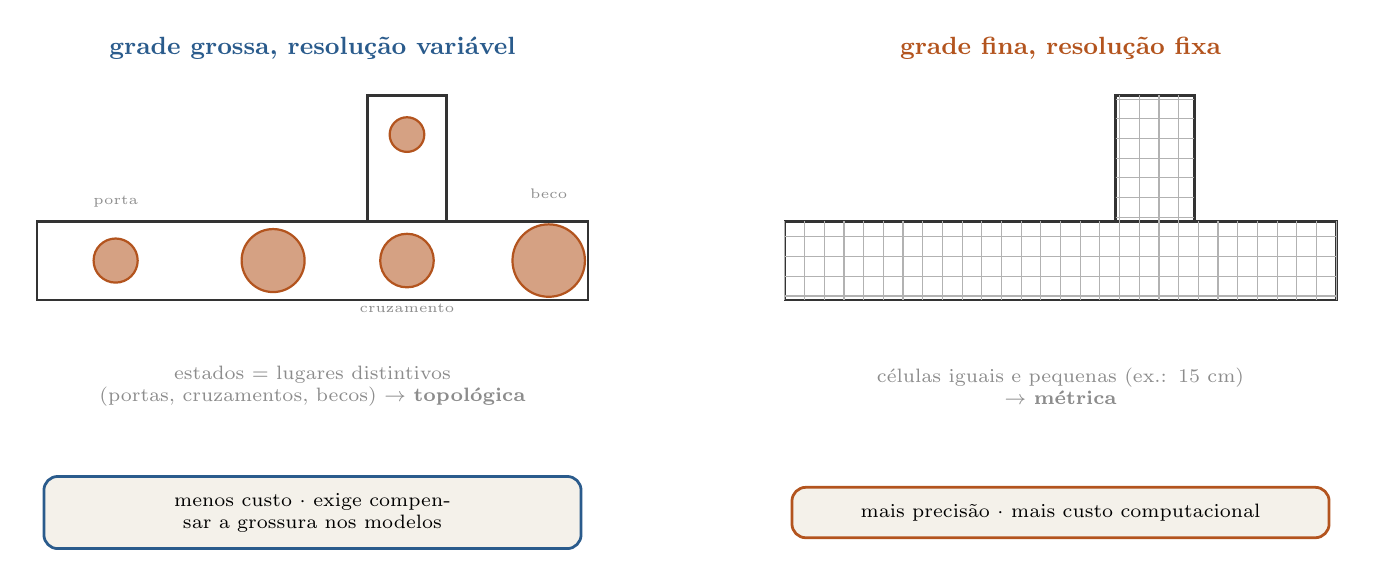
\begin{tikzpicture}[x=1cm,y=1cm]
  % topológica
  \node[font=\small\bfseries, dblue] at (3.5,5.4) {grade grossa, resolução variável};
  \draw[dbody, fill=white, line width=1pt] (0,2.2) rectangle (7,3.2);
  \draw[dbody, fill=white, line width=1pt] (4.2,3.2) rectangle (5.2,4.8);
  \foreach \x/\y/\r/\t in {1.0/2.7/0.28/porta, 3.0/2.7/0.40/{}, 4.7/2.7/0.34/T, 4.7/4.3/0.22/{}, 6.5/2.7/0.46/{fim}} {
    \fill[dorange!55, draw=dorange, line width=0.8pt] (\x,\y) circle (\r);
  }
  \node[dsub, font=\tiny] at (1.0,3.45) {porta}; \node[dsub, font=\tiny] at (4.7,2.1) {cruzamento}; \node[dsub, font=\tiny] at (6.5,3.55) {beco};
  \node[dsub, font=\scriptsize, align=center, text width=7cm] at (3.5,1.1) {estados = lugares distintivos\\ (portas, cruzamentos, becos) $\to$ \textbf{topológica}};
  \node[dbox, rounded corners=5pt, draw=dblue, text width=6.4cm, font=\scriptsize] at (3.5,-0.5) {menos custo $\cdot$ exige compensar a grossura nos modelos};
  % métrica
  \begin{scope}[shift={(9.5,0)}]
    \node[font=\small\bfseries, dorange] at (3.5,5.4) {grade fina, resolução fixa};
    \draw[dbody, fill=white, line width=1pt] (0,2.2) rectangle (7,3.2);
    \draw[dbody, fill=white, line width=1pt] (4.2,3.2) rectangle (5.2,4.8);
    \draw[black!30, line width=0.4pt] (0,2.2) grid[step=0.25] (7,3.2);
    \draw[black!30, line width=0.4pt] (4.2,3.2) grid[step=0.25] (5.2,4.8);
    \node[dsub, font=\scriptsize, align=center, text width=7cm] at (3.5,1.1) {células iguais e pequenas (ex.: 15 cm)\\ $\to$ \textbf{métrica}};
    \node[dbox, rounded corners=5pt, draw=dorange, text width=6.4cm, font=\scriptsize] at (3.5,-0.5) {mais precisão $\cdot$ mais custo computacional};
  \end{scope}
\end{tikzpicture}
\end{document}
